\section{A Proposal To Extend to Distributed-\\Memory Environments}

In the previous sections, we have introduced our implementations on top of BaseX
and the evaluation with a single BaseX server on a dual-CPU system. As
introduced in the original study, data partitioning strategy was studied in a
shared-memory environment, where XML data is stored in a shared memory and can
be concurrently accessible by multiple XPath processors. In the conclusion of
the original paper~\cite{BoLS09},  the authors had pointed out that the
parallelization model is over XML data model, and it can also be adapted to any
XML storage laryout. However,  no matter in the original study, or in our
previous study, the strategies  are applied both in a shared-memory environment. 

Based on our previous experiment results, it would also be promising to use
multiple BaseX servers on multiple CPUs in distributed-memory environments over
large XML documents so that we can exploiting computer clusters to process  them
more efficiently. Then, here comes a question: how we can apply it in a
distributed-memory environment over a number of computers?  In this study, by
exploiting horizontal fragmentation on XML data, we present a  proposal to apply
data partitioning to distributed-memory environments with XML  fragmentation.

\section{Fragmentation}
\subsection{Introduction}

Fragmentation is an effective way to improve scalability of database
systems~\cite{navathe1995mixed, hauglid2010dyfram, khan2010new}.  In the field
of parallel XML processing, there are also some studies on  fragmentation of XML
data~\cite{kling11:dist_xml, KlOD10}.  The most common XML fragmentations are
horizontal fragmentation and vertical fragmentation~\cite{kling11:dist_xml}. Due
to the independence nature of horizontal fragments, it is reletively a more
direct and practical way to work together with data partitioning. We thus focus
on only horizontal fragmentation.

\subsection{Definitions}

To process a large XML document in a distrubed-memory environment,  we first
need to divide an XML document into multiple fragments to be allocated to
multiple computing node for querying. To make the fragments well balanced, we
introduce a fragmentation algorithm with an example in this section.

\subsubsection{Fragment}

To begin with, we give definition to fragment first. In this study, a
\emph{fragment} is a collection of subtrees. Since the main purpose of
fragmentation is to achieve good scalability, we attempt to make our
fragmentation algorithm size-balanced, i.e. to make each fragment have nearly
the same amount of node.  Therefore, a fragment satisfies two condictions.
Firstly, the roots of subtrees in a fragment are consecutive children of a
single  node in the input tree. Secondly, the number of elements in a fragment
is  less than or equal to a given integer \emph{maxsize}.  Let us take the tree
in Fig.~\ref{fig:frag_wholetree} as an example. Let maxsize be 5, then we have
the fragments shown in Figure~\ref{fig:frag_fragmentation}. After applying
horizontal fragmentation to the example XML tree, we obtain eight fragments
enclosed in dotted rectangles.

%Let $D$ = \{$d_1$, $d_2$, ..., $d_n$\} be a collection of document trees such
%that each $d_i \in D$ conforms the same XML schema~\cite{xmlschema}.   Let
%$\mathit{FS}$ = \{$F_1$, $F_2$,..., $F_m$\}  be a collection of fragments such
%that for each $F_i \subset D$. If $\bigcup\limits_{i=1}^{m} F_{i} = F$ and
%$\bigcap\limits_{i=1}^{m} F_{i} = \emptyset$, then $\mathit{FS}$ is a
%\emph{horizontal fragmentation} of $D$.

\begin{figure}[t] 
	\centering
	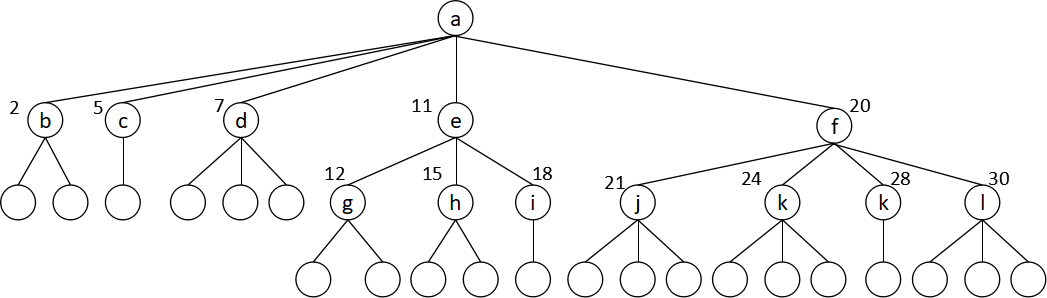
\includegraphics[scale=0.5]{frag_wholetree}
	\caption{An example tree and the PRE values along with nodes}
	\label{fig:frag_wholetree}
	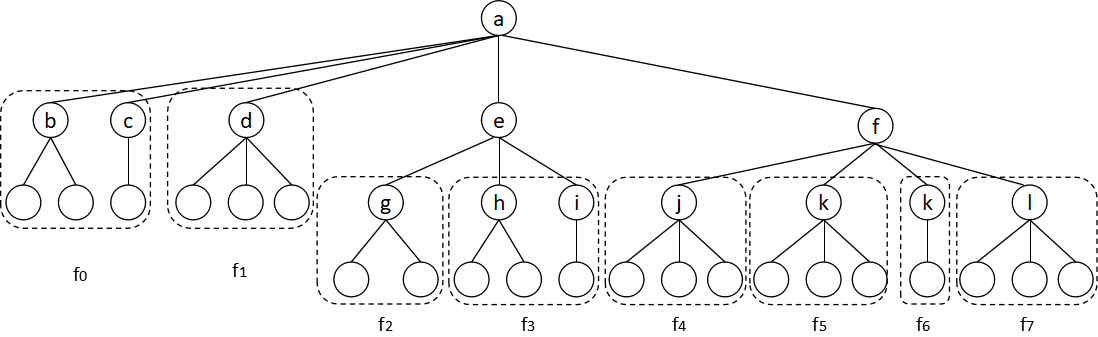
\includegraphics[scale=0.45]{frag_fragmentation}
	\caption{Fragmentation on the example tree given maxsize = 5.}
	\label{fig:frag_fragmentation}	
\end{figure}


\subsubsection{Anchored Fragment}

In order to ease performing top-down XPath queries, we augment each fragment
with a path from the root of the whole tree to the subtrees. We call this
augmented fragment \emph{anchored fragment}. In the running example, we have
eight anchored fragments as shown in Figure~\ref{fig:frag_anchortrees}.

\subsubsection{Root-merged Tree}

In most existing XML database management systems, such as BaseX, it takes a
single XML tree to create an XML database instance. Since a large number of
databases instance arises overheads, we reduce the number of database  instances
by merging some of anchored fragments to \emph{root-merged tree}. A root-merged
tree is a number of anchored fragments merged at the root. we merge the root
node of anchored fragments only, which is enough to make a list of fragments
into a tree. 

To make the merged trees work more size-balanced, we apply the following two
rules to anchored fragments when merging. Firstly, anchored fragments are
randomly grouped. Each group contains a similar number of anchored fragments
and. Then, from each group, a single root-merged tree is created by mering the
root node  of the anchored fragment in the group. Secondly, the anchored
fragments of a root-merged tree are ordered in the original order e.g. document
oder, on purpose of simplifying the process of reordering results.

For the running example, we construct four root-merged trees from eight
fragments with randomization and reodring as shown in
Figure~\ref{fig:frag_mergedtrees}. 

\begin{figure}[t]   
	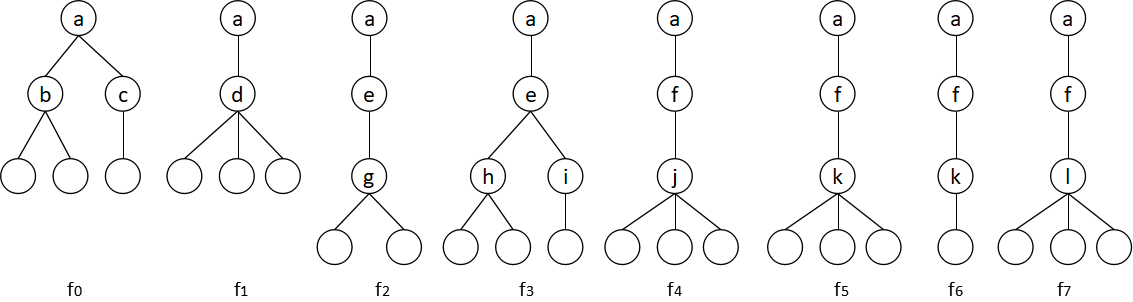
\includegraphics[scale=0.45]{frag_anchortrees}
	\caption{Anchor trees.}
	\label{fig:frag_anchortrees}	
	
	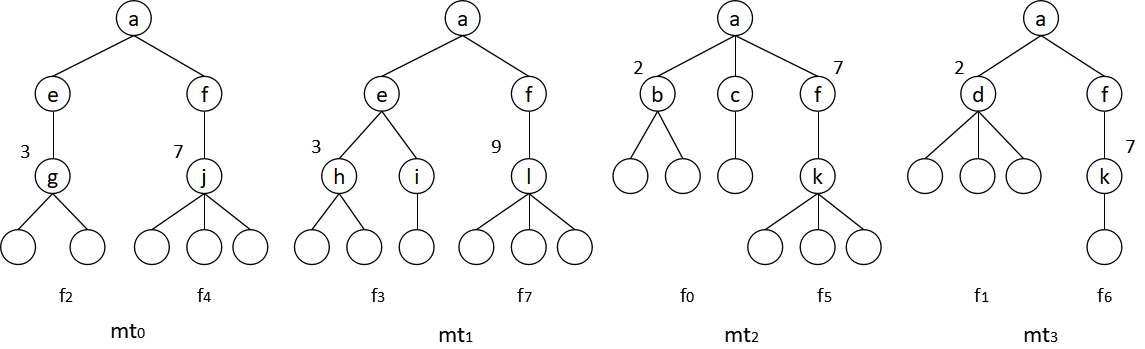
\includegraphics[scale=0.5]{frag_mergedtrees}
	\caption{Root-merged trees.}
	\label{fig:frag_mergedtrees}
\end{figure}


\subsubsection{Fragment Index}

In order to facilitate query evaluation, we design \emph{fragment index} that
is the information required or useful for managing fragments. It has the
following items for each fragment.

\begin{itemize}
	\item fid: fragment ID.
	\item mid: the root-merged tree that has the fragment
	\item mrank: the rank (position) of the fragment in the root-merged tree
	\item size: the size of fragments
	\item gpre: pre-index (in the input tree) of the first element
	\item mpre: pre-index (in the root-merged tree) of the first element
\end{itemize}

For the running example, the fragment index of is created as shown in
Table~\ref{tab:fragmentindex}. 

\begin{table}[t]
	\centering 
	\begin{tabular}{c|c|c|c|c|c}
		\hline
		fid & mid & mrank & size & gpre & mpre \\
		\hline
		0   & mt2 & 0     &   5  & 2    & 2    \\
		1   & mt3 & 0     &   4  & 7    & 2    \\
		2   & mt0 & 0     &   3  & 12   & 3    \\
		3   & mt1 & 0     &   5  & 15   & 3    \\
		4   & mt0 & 1     &   4  & 18   & 7    \\
		5   & mt2 & 1     &   4  & 21   & 7    \\
		6   & mt3 & 1     &   2  & 24   & 7    \\
		7   & mt1 & 1     &   4  & 30   & 9    \\
		\hline
	\end{tabular} 
	\caption{Fragment index.}
	\label{tab:fragmentindex}	
\end{table}

\subsubsection{Pruned Tree}

In our design, we can perform any XPath queries inside of a fragment,  but we
need careful computation for XPath queries that may go out of the  fragment. In
order to perform those XPath queries, we need to know the  global tree structure
in which fragments are located. For this purpose, we construct a \emph{pruned
tree} by replacing the  subtrees with a single node for each fragment. In our
running example, we have a pruned tree as shown in
Figure~\ref{fig:frag_prunedtree}. 

In order to compute the PRE index of the input tree easily, we add \emph{gpre}
for each node. For the nodes representing pruned parts, we add \emph{fid} to
link to the fragmentation index.

\begin{figure}[t]  
	\centering
	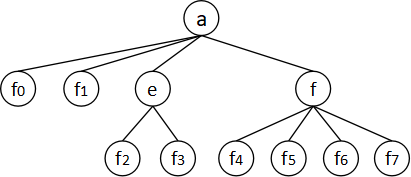
\includegraphics[scale=0.8]{frag_prunedtree}
	\caption{Pruned tree.}
	\label{fig:frag_prunedtree}	
\end{figure}


\subsection{Fragmentation Algorithm}

We assume that all the results lie in the subtrees on the fragment. Thus, to
guarantee the correctness of query results, we need to guarantee the
completeness and uniqueness of nodes such that each node in the input XML tree
is included in at least a fragment. If a node is included a subtree part of a
fragment, then it is not included in any other fragment. 

\begin{figure}[]
	\centering
	\begin{tabular}{l}
		\hline
		\hline
		\makebox[.95\linewidth][l]{\textbf{Algorithm 1} \textsc{Fragmentation}($\mathit{nodes}$, $\mathit{maxsize}$)} \\
		\hline
		\textbf{Input}:           $\mathit{nodes}$: a list of nodes, \\
		\makebox[1em][r]{}\hspace{9 mm}  $\mathit{maxsize} $ : the maximum number of nodes in a fragment \\
		\textbf{Output}: a list of fragments \\
		\makebox[1em][r]{1:}\hspace{1 mm}  $\mathit{fragments} \leftarrow [] $     //a list of fragments \\
		\makebox[1em][r]{2:}\hspace{1 mm}  $fragment \leftarrow \textsc{NewFragment}() $     // create a new fragment \\
		\makebox[1em][r]{3:}\hspace{1 mm}  \textbf{for all} $\emph{node} \in \emph{nodes}$ \textbf{do} \\
		\makebox[1em][r]{4:}\hspace{5 mm}  \textbf{if} \texttt{size($node$)} $ > \mathit{maxsize} $ \textbf{then} \\
		\makebox[1em][r]{5:}\hspace{9 mm}  \textbf{if} $fragment.subtrees.\texttt{size}() > 0$  \textbf{then} \\
		\makebox[1em][r]{6:}\hspace{13 mm} $\mathit{fragments}.Add((\textit{fragment}))$ \\
		\makebox[1em][r]{7:}\hspace{13 mm}  $\mathit{fragment} \leftarrow new \textsc{NewFragment}()$ \\
		\makebox[1em][r]{8:}\hspace{9 mm}  \textbf{end if}\\
		\makebox[1em][r]{9:}\hspace{9 mm}  $\mathit{fragments}.\texttt{AddAll}($\textsc{Fragmentation}$($\texttt{child}$(node), \mathit{maxsize}))$ \\
		\makebox[1em][r]{10:}\hspace{5 mm}  \textbf{else if} \texttt{NodeSize($node$)} + \texttt{NodesSize}$(fragment.subtrees) > \mathit{maxsize}$ \textbf{then} \\
		\makebox[1em][r]{11:}\hspace{9 mm} $\mathit{fragments}.Add(fragment)$ \\
		\makebox[1em][r]{12:}\hspace{9 mm} $\mathit{fragment} \leftarrow  \textsc{NewFragment}()$ \\
		\makebox[1em][r]{13:}\hspace{9 mm} $fragment.subtrees.\texttt{Add}(node)$ \\
		\makebox[1em][r]{14:}\hspace{5 mm}  \textbf{else}\\
		\makebox[1em][r]{15:}\hspace{9 mm} $fragment.subtrees.\texttt{Add}(node)$  \\
		\makebox[1em][r]{16:}\hspace{5 mm}  \textbf{end if}\\
		\makebox[1em][r]{17:}\hspace{1 mm}  \textbf{end for}\\
		\makebox[1em][r]{18:}\hspace{1 mm}  \textbf{for} $i \in [0, \mathit{fragments}.length)$ \textbf{do}\\
		\makebox[1em][r]{19:}\hspace{5 mm}  $\mathit{fragments}[i] \leftarrow $\texttt{AddPath}($\mathit{fragments}[i]$)  \\
		\makebox[1em][r]{20:}\hspace{1 mm}  \textbf{end for}\\
		\makebox[1em][r]{21:}\hspace{1 mm}  \textbf{return} $\mathit{fragments}$\\
		\hline
	\end{tabular}
	\caption{The fragmentation algorithm.}
	\label{fig:algQuery1}
\end{figure}


\begin{figure}[]
	\centering
	\begin{tabular}{l}
		\hline
		\hline
		\makebox[.95\linewidth][l]{\textbf{Algorithm 2} \textsc{MakeAnchoredFragment}($\mathit{fragment}$)} \\
		\hline
		\textbf{Input}:   $\mathit{fragment}$: a fragment\\
		\textbf{Output}:  an anchored fragment augmented with the \\
		\makebox[1em][r]{}\hspace{13 mm}  path to the root of the whole tree\\
		\makebox[1em][r]{1:}\hspace{1 mm}  $\mathit{p} \leftarrow $\texttt{parent}$(fragment.subtrees[0]) $   \\
		\makebox[1em][r]{2:}\hspace{1 mm}  $node \leftarrow $ \texttt{clone}($p$)    \\
		\makebox[1em][r]{3:}\hspace{1 mm}  $node.addChildren(subtrees) $ \\
		\makebox[1em][r]{4:}\hspace{1 mm}  \textbf{while} \texttt{parent}$(p) \neq \mathit{NULL}$ \textbf{do}\\
		\makebox[1em][r]{5:}\hspace{5 mm}  $p \leftarrow $ \texttt{parent}($p$) \\
		\makebox[1em][r]{6:}\hspace{5 mm}  $tempnode \leftarrow$ \texttt{clone}($p$)  \\
		\makebox[1em][r]{7:}\hspace{5 mm}  $tempnode.addChild(node)$ \\
		\makebox[1em][r]{8:}\hspace{5 mm}  $node \leftarrow tempnode$ \\
		\makebox[1em][r]{9:}\hspace{1 mm}  \textbf{end while} \\
		\makebox[1em][r]{10:}\hspace{1 mm} $fragment.root \leftarrow node$\\
		\makebox[1em][r]{11:}\hspace{1 mm}  \textbf{return} $\mathit{fragment}$\\
		\hline
	\end{tabular}
	\caption{Add path to a list of subtrees to create a anchored fragment}
	\label{fig:algQuery2}
\end{figure}


  
Algorithm 1 describes how our fragmentation works to apply a horizontal
fragmentation to an input tree. The arguments of input are a list of nodes
denoting the tree to be fragmented and an integer number denoting the maximum
number of nodes a fragment can have.  In Line 1--2, we declare an empty list of
fragments and a new fragment for holding results. In Line 3--17, we traverse
nodes in the input list to generate fragments. If a node have more number of
descendant nodes greater than maxsize, we apply the fragmentation iteratly on
the children of the node (Line 4--9) and add the results into $fragments$. If
not, we check the total number of descendant nodes in $fragment.subtrees$ and
the $node$ excesses maxsize, we save the current fragment and put the current
node into a new fragment (Line 10--13). Otherwise, the current node is added to
$fragment.subtrees$ as one of the subtrees in the current fragment. After the
iteration, we obtain a list of fragments, each of which contains a list of
subtrees. We add the last use Algorithms 2 to create anchored fragments by
adding the path from the current subtrees to the root of the original tree (Line
18--20). In Algorithm 2, we basically keep looking upward, to add all the
ancestor nodes to the current fragment.

There are also several functions used in Algorithms 1 and 2. We describe 
them as below:

\begin{itemize}
	\item \texttt{NodeSize($node$)} returns the number of descendants of $node$, 
	where node is a single node. 
	\item \texttt{NodesSize($nodes$)} returns the sum of number of descendants 
	of each node in $nodes$, where $nodes$ is a list of nodes. 
	\item \texttt{child($node$)} returns the children of $node$.
	\item \texttt{parent($node$)} returns the parent of $node$. 
	\item \texttt{clone($node$)} returns a node cloned from $node$. The function create
	an empty node and copy the name and attributes from $node$.
\end{itemize}

\section{Our Distributed XPath Query Framework}

We design an XPath query framework using horizontal fragmentation with data
partitioning strategy on top of BaseX over a distributed-memory environment.  In
this framework, there are one master and $N_s$ workers. The master is a computer
running a Java program that is the implementation of our query algorithm. It
works for sending queries to all workers and processing results returned from
them. A worker is a computer that runs a BaseX server in charge of evaluating
received queries.  After fragmentation, the fragments are mapped to workers. For
each workers, a root-merged tree is assigned and accordingly a database instance
will be created on every worker. Then, queried are evaluated on them  and the
results returned from all the workers will be merged on the master. To compare
with, we introduce both cases that the data partiationing starategies is used or
not. The one with our data partitioning is the regular query and the other is
with data partitioning. 

\subsection{Query Rewriting}

An input XPath query is rewritten into an XQuery expression to be then processed
by BaseX workers. The rewriting is different depending on whether data
partitioning strategy is used or not.

\subsubsection{Regular Query}
\label{no-dps}

Since the nodes in the results will no long follow the original order in the
input document, we return the nodes along with their PRE index for later
identifying and reordering by using the following expression.

\verb|for $node in db:open(`db')$query|\\
\verb|     return ((`', db:node-pre($node)), $node)|
\footnote{\texttt{return (a, b)} will add a line break between \texttt{a} and
	\texttt{b} while returning.}

We separate the PRE value and the content of a node by a linebreak and add an
extra linebreak among resultant nodes.

\subsubsection{Query with Data Partitioning}

When applying data Partitioning, we use the server-side implementation. In
order to maintain the order of resultant nodes, we make some change to the
server-side implementation. For the two-phases implementation, we do not need to
change the first phase, which still returns the PRE values of the results of
prefix query. We need to change the second phase, where the \verb|return|
statement in the suffix query needs to be modified to 
\verb|return ((`',db:node-pre($node)), $node)|, 
i.e. the same as the XQuery expression described in~\ref{no-dps}.



\subsection{Evaluating Queries}

The evaluation an XPath queries consists of two steps: sending query and
processing results. 

After an input query being rewritten, it will be sent form the master to all
srevers for executing. After sending, the master will be idle waiting for
results to be sent back.

\subsection{Processing Results}

The results are returned from all servers through the network (some workers may
return empty results). There are two issues we need to consider when processing
results. First, since the size of results can be larger than the memory size of
the master (such as XM1 that returns about 90 the size of the input data), we
thus store results on disk. Second, due to the randomization, the results
returned from all workers are not in the original order. Thus, we have to
recover the original order of results when processing. It is different to deal
with the order depending on whether data partitioninng strategy is used.

\subsubsection{Regular Query}

First, since we have the PRE values of resultant nodes, we can use them to
determine which fragment a resultant node belongs to by comparing with the
$mpre$ of each fragment, where $mpre$ is the PRE value of the root of the first
subtree in the fragment. Given a list of fragments $F$ = \{$f_0$, $f_1$,...,
$f_n$\}, a function \textsc{GetMpre($f$)} that returns the $mpre$ of the
fragment $f$ and the PRE value $pre$ of a node $n$, if \textsc{GetMpre($f_i$)}
$\leq pre <$ \textsc{GetMpre($f_{i+1}$)}, ($i  < n$ - 1) or
\textsc{GetMpre($f_i$)}$\leq pre$, ($i = n$ - 1), then $n$ belongs to $f_i$. For
example, there are three fragments, and their $mpre$ are 3, 10, 20 respectively.
A node with the PRE value 5 belongs to the first fragment. Note that we do not
need to deal with the order of the nodes in the same fragment, because these
nodes in the same fragment still keep the original order. Thus, the results can
be grouped by fragments.

Next, we store the results in a list of files, each of which stores the results
that belong to the same fragment. We use fragment id to name these files so
that we can obtain the results stored in these files in the original order, when
reading the files ordered by their names

Through the above method, since all the fragment can be processed separately, we
can receive the results and save them to disk in parallel.

\subsubsection{Query with Data Partitioninng}

Since data partitioninng strategy uses multiple processors, results of the same
fragment may be processed by two processors. For example, when we use two
processes $p_1$ and $p_2$ to process the same merged tree with only one fragment
$f_0$, the resultant nodes in the fragment may be processed by both processors.
Since there is only one file that corresponds the fragment for storing, the two
processor cannot write the resutls to the file at the same time.

There are two ways to solve the problem. One way is to write the results in
sequential, i.e. we let only one processor to write at a time. For example, we
let $p_1$ write first then $p_2$ follows. However, this way should be slow, because
when a processor is writing results, the following processors have to wait.
Another way is simply to add a suffix to the file names then concatenate files
with suffix. For the above example, $p_0$ changes the file name to
\texttt{0\_start.txt} and $p_1$ to \texttt{0\_end.txt} for the fragment $f_0$.
After receiving all the results, we concatenate the two files to \texttt{0.txt}.
In this way, we can still process the results in parallel. But in some extreme
case when the results of a fragment is very larger, the concatenation may bring
significant overhead.

